\documentclass{article}

\usepackage[a4paper, total={6in, 8in}]{geometry}
\usepackage[english, lithuanian]{babel}
\usepackage{float}
\usepackage{amsmath}
\usepackage{subcaption}
\usepackage{datetime}
\usepackage{comment}
\usepackage{caption}
\usepackage{graphicx}
\usepackage{amsfonts}
\usepackage{listings}
\usepackage{parskip}
\usepackage{amssymb}
\usepackage[T1]{fontenc}
\usepackage{url}
\usepackage{xcolor}
\usepackage{hyperref}

\DeclareUnicodeCharacter{2212}{-}
\selectlanguage{lithuanian}

\definecolor{backcolour}{rgb}{0.95,0.95,0.92}
\definecolor{codegreen}{rgb}{0,0.6,0}

\lstdefinestyle{myStyle}{
    backgroundcolor=\color{backcolour},   
    commentstyle=\color{codegreen},
    basicstyle=\ttfamily\footnotesize,
    breakatwhitespace=false,         
    breaklines=true,                 
    keepspaces=true,                 
    numbers=left,       
    numbersep=5pt,                  
    showspaces=false,                
    showstringspaces=false,
    showtabs=false,                  
    tabsize=2,
    literate={ą}{{\k{a}}}1
           {Ą}{{\k{A}}}1
           {č}{{\v{c}}}1
           {Č}{{\v{C}}}1
           {ę}{{\k{e}}}1
           {Ę}{{\k{E}}}1
           {ė}{{\'{e}}}1
           {Ė}{{\'{E}}}1
           {į}{{\'{i}}}1
           {Į}{{\'{I}}}1
           {š}{{\v{s}}}1
           {Š}{{\v{S}}}1
           {ų}{{\k{u}}}1
           {Ų}{{\k{U}}}1
           {ū}{{\={u}}}1
           {Ū}{{\={U}}}1
           {ž}{{\v{z}}}1
           {Ž}{{\v{Z}}}1   
}
\lstset{style=myStyle}

\begin{document}
\newlength{\mywidth}
\settowidth{\mywidth}{Darbo vadovas:}
\begin{titlepage}
    \vskip 20pt
    \centerline{\bf \large VILNIAUS UNIVERSITETAS}
    \bigskip
    \centerline{\large \textbf{MATEMATIKOS IR INFORMATIKOS FAKULTETAS}}
    \vskip 120pt
    \centerline{\bf \Large \textbf{Laboratorinis darbas 1}}
    \vskip 50pt
    \begin{center}
        {\bf \LARGE Vienmatis optimizavimas}
    \end{center}
    \bigskip
    \bigskip
    \centerline{\Large Nikita Gainulin}
    \vskip 90pt
    \vskip 200pt
    \centerline{\large \textbf{VILNIUS 2024}}
\end{titlepage}

\tableofcontents

\clearpage
\section{Tikslo funkcija}
Visi šioje ataskaitoje minėti metodai bus pritaikyti šiai tikslo funkcijai:
\begin{equation}\label{eq:1}
    f(x) = \frac{(x^2-5)^2}{7}-1
\end{equation}
Mano \lstinline|Python| kode aprašyta taip:
\lstinputlisting[language=Python]{fx.py}
\section{Vienmačiai optimizavimo metodai ir jų algoritmai}
\subsection{Intervalo dalijimo pusiau metodas}
Pirmiausia reikia nustatyti intervalą, kuriame ieškosime minimumo taško. Minėto intervalo ribas įsiminsime kintamaisiais \textit{l} (kairioji riba) ir \textit{r} (dešinioji riba). Pradiniame intervale pasirenkam tris bandymo taškus $x_{1}$, $x_{2}$ ir $x_{m}$, taip, kad $x_{m}$ būtų intervalo vidurio taškas, o $x_{1}$ ir $x_{2}$ tarp \textit{l} ir vidurio taško bei \textit{r} ir vidurio taško atitinkamai. Tada apskaičiuojame $f(x_{m})$, $f(x_{1})$ ir $f(x_{2})$ reikšmes. Po to palyginame gautas reikšmes, t. y. kuriame taške funkcija įgyja didesnę reikšmę. Tas taškas ir nustato intervalą, kurį reikia atmesti. Kadangi ieškome minimumo taško, atmetamas atitinkamas intervalas, atitinkmai keičiami $x_{1}$, $x_{2}$ ir $x_{m}$ taškai bei perskaičiuojami $f(x_{m})$, $f(x_{1})$ ir $f(x_{2})$ reikšmės. Algoritmas tęsiamas tol, kol gaunamas pakankamai tikslus minimumo taškas, t.y. kol intervalo ilgis $r-l$ nėra mažiau už tam tikrą $\varepsilon$ reikšmę.

Štai kaip tai atrodo mano \lstinline|Python| kode:
\lstinputlisting[language=Python]{halfcut.py}
Vizualizuojant mūsų tikslo funciją (\ref{eq:1}) šiuo metodu gauname štai tokį grafą:
\begin{figure}[H]
    \centering
    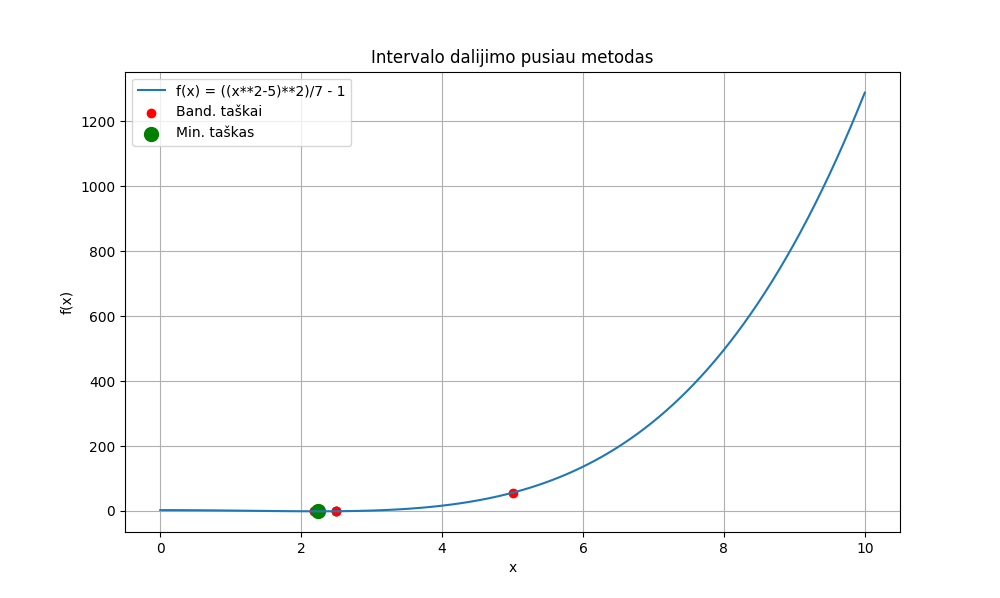
\includegraphics[width=1\textwidth]{Figure_1.png}
    \caption{Intervalo dalijimo pusiau metodo vizualizacija (\ref{eq:1}) tikslo funkcijai.}
    \label{fig:1}
\end{figure}
\subsection{Auksinio pjūvio metodas}
Šis metodas yra labai panašus į intervalo dalijimo pusiau metodą, tačiau per kiekvieną iteraciją naudojami tik 2, o ne 3 bandomieji taškai. Mums vis dar reikia pasirinkti intervalą ir įsiminti jo kairiąją \textit{l} ir dešiniąją \textit{r} ribas, tačiau šį kartą $x_{1}$ ir $x_{2}$ apskaičiuojami kitaip, naudojant \textit{Fibonačio} reikšmę, kuri apytiksliai lygi:
\begin{equation*}
    \tau = \frac{\sqrt{5}-1}{2} \approx 0.61803...
\end{equation*}
Apskaičiavę $x_{1}=r-\tau(r-l)$ ir $x_{2}=l+\tau(r-l)$ taškus, apskaičiuojame funkcijos reikšmes $f(x_{1})$ ir $f(x_{2})$ šiuose taškuose. Po to dar kartą palyginame funkcijos reikšmes ir pašaliname intervalus pagal didesnę vertę, perskaičiuojame taškus ir naujas funkcijos reikšmes ir kartojame tuos pačius veiksmus kiekvieną iteraciją, kol vėl gauname pakankamai tikslų minimumo tašką.

Algoritmo \lstinline|Python| kodas:
\lstinputlisting[language=Python]{goldratio.py}
Vizualizuojant mūsų tikslo funciją (\ref{eq:1}) šiuo metodu gauname štai tokį grafą:
\begin{figure}[H]
    \centering
    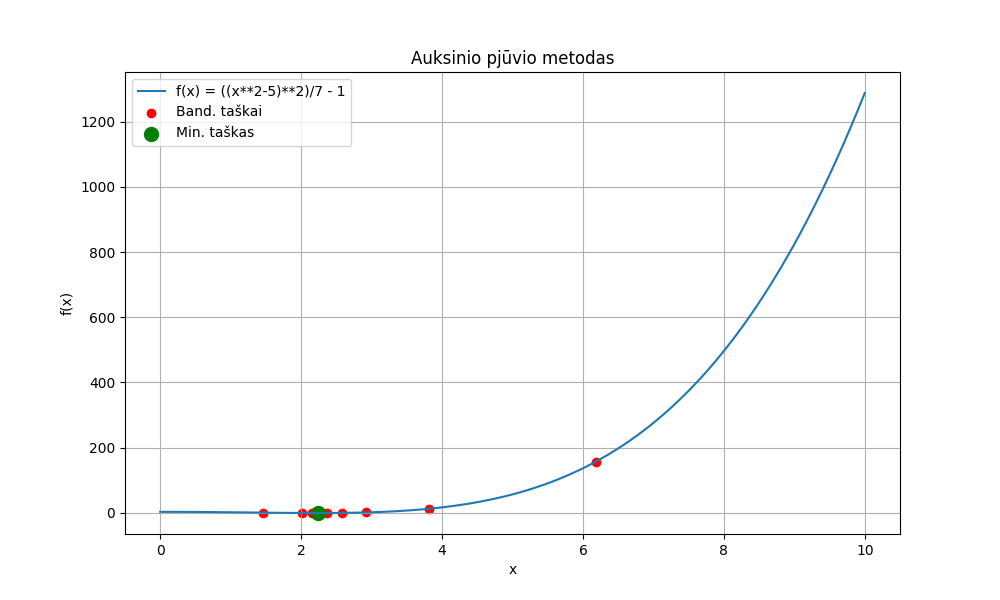
\includegraphics[width=1\textwidth]{Figure_2.png}
    \caption{Auksinio pjūvio metodo vizualizacija (\ref{eq:1}) tikslo funkcijai.}
    \label{fig:2}
\end{figure}
\subsection{Niutono metodas}
Skirtingai nuo dviejų ankstesnių metodų, kurie remiasi konkretaus intervalo pjovimu, Niutono metodas remiasi vienu pradiniu tašku $x_{i}$ ir Teiloro eilutėmis iki antros eilės. Pasirinkus pradinį tašką $x_{i}$, kitas taškas apskaičiuojamas pagal šią formulę:
\begin{equation}\label{eq:2}
    x_{i+1} = x_{i} - \frac{f'(x_{i})}{f''(x_{i})}
\end{equation}
Tokiu būdu iteracija po iteracijos taškas artėja prie minimumo.

Vienas įdomus faktas, kurį pastebėjau, yra tai, kad daugelyje internetinių šaltinių kaip Niutono metodo pagrindas naudojama ši formulė:
\begin{equation*}
    x_{i+1} = x_{i} - \frac{f(x_{i})}{f'(x_{i})}
\end{equation*}
Nors ši formulė paprastai naudojama dažniau ir bendriau, formulė (\ref{eq:2}) yra tikslesnė optimizavimo kontekste, todėl ją ir naudojame vietoj šios bendrosios formulės.

Algoritmo \lstinline|Python| kodas:
\lstinputlisting[language=Python]{newton.py}
Vizualizuojant mūsų tikslo funciją (\ref{eq:1}) šiuo metodu gauname štai tokį grafą:
\begin{figure}[H]
    \centering
    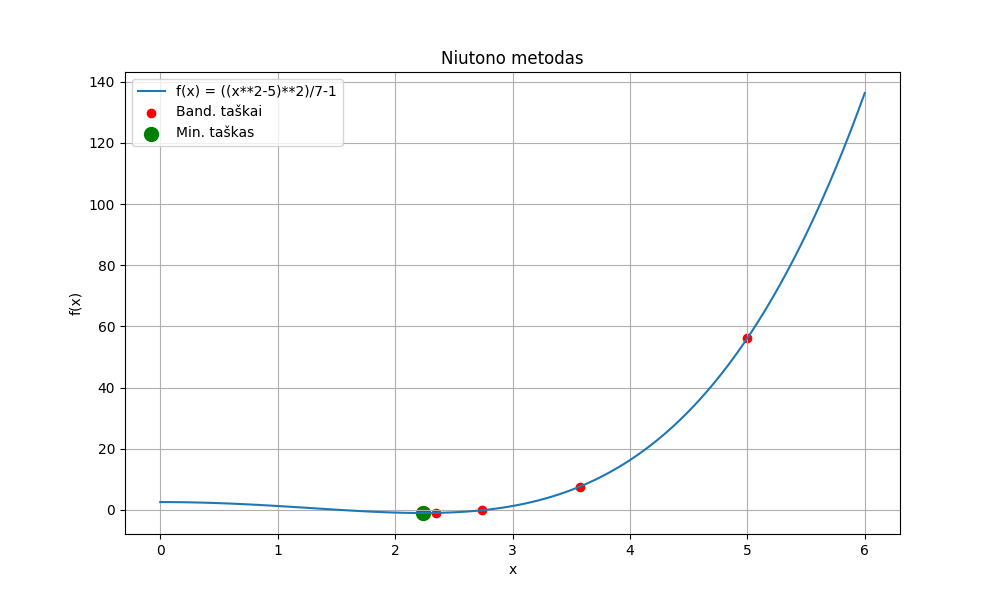
\includegraphics[width=1\textwidth]{Figure_3.png}
    \caption{Niutono metodo vizualizacija (\ref{eq:1}) tikslo funkcijai.}
    \label{fig:3}
\end{figure}
\section{Rezultatai ir jų palyginimai}
\subsection{Minimumo taškas ir funkcijos reikšmė tame taške}
Kaip ir galima tikėtis, taikant visus metodus gaunami daugiau ar mažiau panašūs rezultatai:
\begin{table}[H]
    \centering
    \begin{tabular}{|p{3cm}|p{3cm}|p{3cm}|p{3cm}|}
    \hline
    \multicolumn{1}{|l|}{} & Intervalo dalijimo pusiau metodas & Auksinio pjūvio metodas & Niutono metodas \\ \hline
                       Minimumo taškas    & 2.236061 & 2.236057 & 2.236105 \\ \hline
                       F-jos reikšmė   & -0.999999 & -0.999999 & -0.999999 \\ \hline
    \end{tabular}
\end{table}
Matomas šiek tiek didesnis Niutono metodo minimumo taško nuokrypis nuo kitų metodų. Tačiau tai nebūtinai yra blogai, tiesiog rodo, kad Niutono metodo tikslumas priklauso nuo tokių parametrų kaip pradinis taškas ir funkcijos pobūdis, t.y. ar pati funkcija lygi, turi „staigių posūkių ar kampų“, kvadratinė, logaritminė ir t.t.
\subsection{Greitis}
Pirmiausia turėtume nustatyti tikslią greičio prasmę optimizavimo metodų algoritmų kontekste. Mūsų atveju \textbf{greitis} - tai kiekvieno algoritmo vidinių iteracijų kiekis, per kurį randamas tikslus minimumo taškas (arba intervalas, kuris yra mažesnis už iš anksto nustatytą $\varepsilon$). Paprastai kuo mažiau iteracijų algoritmui reikia minėtam mažiausiam taškui pasiekti, tuo jis yra greitesnis. Žinoma, tai nebūtinai reiškia, kad minėtas algoritmas yra efektyvesnis, kaip pamatysime šiek tiek vėliau, tačiau griežtai kalbant tik apie greitį, atsižvelgiame tik į iteracijų skaičių.

Apskaičiavę kiekvieno algoritmo iteracijų skaičių mūsų tikslo funkcijai (\ref{eq:1}), gauname tokį rezultatą:
\begin{table}[H]
    \centering
    \begin{tabular}{|p{3cm}|p{3cm}|p{3cm}|p{3cm}|}
    \hline
    \multicolumn{1}{|l|}{} & Intervalo dalijimo pusiau metodas & Auksinio pjūvio metodas & Niutono metodas \\ \hline
                       Iteracijų skaičius    & 17 & 24 & 6 \\ \hline
    \end{tabular}
\end{table}
Kaip matome, iš trijų metodų Niutono gali būti laikomas greičiausiu mūsų tikslo funkcijai (\ref{eq:1}). Tai nestebina, nes naudodamas pirmos ir antros eilės išvestines Niutono metodas minimumo taško link žengia daug didesniais žingsniais, priešingai nei intervalo dalijimo pusiau ir auksinio pjūvio metodai, kurie, naudodami tam tikrus intervalus, prie jo artėja lėčiau. Skirtumas tarp kitų dviejų metodų taip pat gana tikėtinas, nes intervalo dalijimo pusiau metodas, kaip rodo pavadinimas, per kiekvieną iteraciją intervalą sumažina perpus, o auksinio pjūvio metodas perkelia 61.8\% ankstesnės iteracijos intervalo (nes $\tau \approx 0.61803...$), t. y. per kiekvieną iteraciją jis atmeta tik 38.2\% intervalo, o tai akivaizdžiai mažiau nei pusė.

Taigi, apskritai kalbant apie metodų greitį mūsų tikslo funkcijai, rezultatai yra gana tikėtini: Niutono metodas yra greičiausias, auksinio pjūvio - lėčiausias, intervalo dalijimo pusiau - tarp jų.
\subsection{Efektyvumas}
Optimizavimo metodų algoritmų \textbf{efektyvumas} - tikslo funkcijos iškvietimų kiekis. Kuo mažiau kartų iškviečiame funkciją tam tikro taško reikšmei apskaičiuoti, tuo mažiau išteklių sunaudojame algoritmui vykdyti, vadinasi, tuo efektyviau naudoti tam tikrą metodą. Vėlgi svarbu pažymėti, kad efektyvumas ir greitis remiasi skirtingais rodikliais (atitinkamai tikslo funkcijos iškvietimų kiekiu ir iteracijų kiekiu) ir yra visiškai nepriklausomi, todėl jei metodas yra greičiausias, jis nebūtinai yra efektyviausias, ir atvirkščiai.

Apskaičiavę kiekvienam algoritmui mūsų tikslo funkcijos (\ref{eq:1}) iškvietimų kiekį, gauname tokius rezultatus:
\begin{table}[H]
    \centering
    \begin{tabular}{|p{3cm}|p{3cm}|p{3cm}|p{3cm}|}
    \hline
    \multicolumn{1}{|l|}{} & Intervalo dalijimo pusiau metodas & Auksinio pjūvio metodas & Niutono metodas \\ \hline
                    Tikslo f-jos iškvietimų skaičius & 35 & 26 & 12 \\ \hline
    \end{tabular}
\end{table}

Atrodo, kad mūsų atveju Niutono metodas taip pat yra efektyviausias iš trijų. Tai galima paaiškinti tuo, kad mūsų pradinis spėjimas nėra labai toli nuo tikrojo minimumo taško, taip pat tuo, kad kvadratinė tikslo funkcija yra gana sklandi ir neturi tiek daug „staigių posūkių“. Tikriausiai matytume kitokį vaizdą, jei, tarkime, mūsų pradinis spėjimas būtų 100 arba funkcija būtų trigonometrinė. Tačiau kai kalbama apie kitus du metodus, matome visiškai priešingą vaizdą, nei matėme greičio kontekste. Šį kartą auksinio pjūvio metodas yra efektyvesnis su 26 tikslo funkcijos iškvietimais, nei intervalo dalijimo pusiau su 35. Tai galima paaiškinti tuo, kad pirmasis metodas turi tik 2 taškus kaip intervalų skaičiavimus lemiančius veiksnius - $x_{1}$ ir $x_{2}$, o antrasis - 3 taškus: $x_{1}$, $x_{2}$ ir $x_{m}$. Akivaizdu, kad su kuo mažiau taškų turi dirbti metodai - tuo mažiau tikslo funkcijos iškvietimų bus atlikta, o tai atsispindi bendrame kiekvieno metodo efektyvume.

Apibendrinant, efektyviausias metodas mūsų tikslo funkcijai (\ref{eq:1}) būtų Niutono, po jo seka auksinio pjūvio, o neefektyviausias - intervalo dalijimo pusiau.
\section{Išvada}
Šio darbo tikslas buvo parašyti kiekvieno iš minėtų vienmačių optimizavimo metodų algoritmą, palyginti jų rezultatus ir juos vizualizuoti, taip pat palyginti jų greitį bei efektyvumą. Baigdamas norėčiau atkreipti dėmesį į šiuos du savo pastebėjimus: pirma, kalbant apie optimizavimo metodų algoritmų greitį ir efektyvumą, jie yra visiškai nepriklausomi ir gali nekoreliuoti tarp metodų, kaip matyti iš intervalo dalijimo pusiau ir aukso pjūvio metodų pavyzdžio. Antra, kalbant konkrečiai apie Niutono metodą, nors mūsų scenarijaus atveju jis iš tiesų pasirodė greičiausias ir efektyviausias, mano nuomone, tai nereiškia, kad jis veiks taip pat ir daugeliu kitų atvejų. Jau anksčiau nustačiau, kad metodui iš tikrųjų reikia, kad pradinis spėjimas būtų kuo artimesnis minimaliam taškui, taip pat kad pati tikslo funkcija būtų kuo tolygesnė.
\section{Priedas}
Pilnas \lstinline|Python| kodas:
\lstinputlisting[language=Python]{Nikita_Gainulin_lab1.py}

Tiesioginė nuoroda atsisiųsti: \href{https://www.dropbox.com/scl/fi/kn1geotq32bo3muggn7q3/Nikita_Gainulin_lab1.py}{čia} arba \url{https://www.dropbox.com/scl/fi/kn1geotq32bo3muggn7q3/Nikita_Gainulin_lab1.py}


\end{document}